\documentclass[12pt,a4paper]{amsart}
\usepackage{a4wide}
\usepackage[utf8]{inputenc}
\usepackage[T2A]{fontenc}
\usepackage{graphics,graphicx,epsfig}
\usepackage{amssymb,amsfonts,amsthm,amsmath,mathtext,cite,enumerate,float}
\usepackage[english,russian]{babel}
\usepackage[all]{xy}
\usepackage{morefloats}
\usepackage{pgf}
\usepackage[debug,outputdir={docgraphs/}]{dot2texi}
\usepackage{tikz}
\usepackage{scalefnt}
\usepackage{listings}
\usepackage{float}
\usetikzlibrary{shapes,arrows}
\usetikzlibrary{decorations.pathmorphing}

% Comment the following block when compiling this .tex with a saner compiler than texlive.
\makeatletter
\def\@settitle{\begin{center}%
    \baselineskip14\p@\relax
    \bfseries
    \@title
  \end{center}%
}
\makeatother

\newtheorem{algo}{Алгоритм}
\newtheorem{stat}{Утверждение}
\newtheorem{defin}{Определение}

\begin{document}
% Comment the following block when compiling this .tex with a saner compiler than texlive.
\pagestyle{plain}
\lstset{language=C++}

\title{Алгоритмы порождения допустимых суперпозиций существенно нелинейных моделей}
\author{Г.\,И.~Рудой}
\address{Московский физико-технический институт, ФУПМ, каф. <<Интеллектуальные системы>>}
\thanks{Научный руководитель В.\,В.~Стрижов}

\begin{abstract}
  При восстановлении нелинейной регрессии предлагается рассмотреть набор
  индуктивно порожденных моделей с целью выбора оптимальной модели. В работе
  исследуются индуктивные алгоритмы порождения допустимых существенно
  нелинейных моделей. Предлагается алгоритм, порождающий все возможные
  суперпозиции заданной сложности за конечное число шагов, и приводится его
  теоретическое обоснование. В вычислительном эксперименте приводятся
  результаты для задачи моделирования волатильности опционов.
\end{abstract}
\keywords{Символьная регрессия, нелинейные модели, индуктивное порождение нелинейных моделей, волатильность опционов}

\maketitle

\section{Введение}

В ряде приложений \cite{Barmpalexis201175, Shi:2011:CRM, DOI:10.1504/IJCENT.2010.038358}
возникает задача восстановления регрессии по набору измеренных данных с
условием возможности проинтерпретировать полученные данные экспертом.

Одним из методов, позволяющих получать интерпретируемые модели, является
символьная регрессия \cite{davidson:2000:snrea, reference/ml/X10vc},
в ходе которой измеренные данные приближаются некоторой математической
формулой, например, $ \sin x^2 + 2x $ или $\log x - \frac{e^x}{x} $.
В ходе работы символьной регрессии данные приближаются различными формулами,
являющимися произвольными суперпозициями функций из некоторого заданного
набора. Одна из возможных реализаций этого метода
предложена Джоном Коза \cite{Koza1998GP, Koza1998Intro}, использовавшим
эволюционные алгоритмы для реализации символьной регрессии. Иван Зелинка
предложил дальнейшее развитие этой идеи \cite{Zelinka2008}, получившее
название аналитического программирования.

Алгоритм построения требуемой математической модели выглядит следующим образом:
дан набор примитивных функций, из которых можно строить различные формулы
(например, степенная функция, $+$, $\sin$, $\tan$). Начальный набор формул
строится либо произвольным образом, либо на базе некоторых предположений
эксперта. Затем на каждом шаге производится оценка каждой из формул согласно
функции ошибки либо другого \footnote{Сходу не нашел публикаций на тему
использования других функционалов. Похоже, у Владиславлевой что-то было, но
пока не могу сослаться на что-то конкретное.} функционала качества. На базе
этой оценки у некоторой части формул случайным образом заменяется одна элементарная
функция на другую (например, $\sin$ на $\cos$ или $+$ на $\times$), а у некоторой
другой части происходит взаимный попарный обмен подвыражениями в формулах.

Получаемая формула является математической моделью \cite{Pavlovsky2000}
исследуемого процесса или явления --- то есть, это математическое отношение,
описывающее основные закономерности, присущие этому явлению.

Среди возможных путей улучшения качества символьной регрессии --- анализ
информативности различных признаков. Например, в ходе работы эволюционного
алгоритма можно выявлять, какие из параметров слабо влияют на качество
получающейся формулы, и либо убирать их совсем, либо обеспечивать
неслучайность замены элементарных функций или обмена поддеревьев с целью
замены этих параметров на другие в предположении, что они, возможно,
окажутся более информативными.

Целью данной работы является теоретическое обоснование алгоритмов индуктивного
порождения моделей и анализ этих алгоритмов.

Другим вопросом, возникающим при применении подобных эволюционных алгоритмов,
является их принципиальная теоретическая корректность: способен ли вообще
такой алгоритм породить искомую формулу.

Алгоритм индуктивного порождения моделей, предложенный в настоящей работе, решает
некоторые типичные проблемы предложенных ранее методов, упомянутые, например,
в \cite{Zelinka2008}, а именно:
\begin{itemize}
  \item Порождение рекурсивных суперпозиций, суперпозиций, содержащих
	несоответствующее используемым функциям число аргументов, и т. д. --- в
	предложенном алгоритме эти проблемы не возникают по построению.
  \item Проблемы с областью определений и/или значений.
  \item При ограничении числа примитивных функций, участвующих в суперпозиции,
	а также при соответствующем задании множества примитивных функций
	исключается проблема слишком сложных суперпозиций.
\end{itemize}

В части 2 данной работы формально поставлена задача построения алгоритма
индуктивного порождения моделей. Затем, в части 3 строится искомый алгоритм
для частного случая непараметризованных моделей и доказывается его корректность,
а затем алгоритм обобщается на случай моделей, имеющих параметры. В части 4
описываются вспомогательные технические приемы, использованные в практическом
алгоритме порождения моделей, описанном в части 5.

\section{Постановка задачи}

\subsection{Алгоритмическая часть}

Пусть дана регрессионная выборка:
\[
D = \{ (\mathbf{x_i}, y_i) \mid i \in \{1, \dots, N\},
			\mathbf{x_i} \in \mathbb{X} \subset \mathbb{R}^n,
			y_i \in \mathbb{Y} \subset \mathbb{R} \}.
\]
Требуется построить аналитическую функцию $f : \mathbb{R}^n \rightarrow \mathbb{R}$ из
заданного множества элементарных функций $G$ и доставляющую минимум
некоторому функционалу ошибки.

То есть, если множество всех суперпозиций:
\[
\mathcal{F} = \{ f_r \mid
			f_r : (\boldsymbol{\omega}, \mathbf{x}) \mapsto \mathbb{Y},
			r \in \mathbb{R} \},
\]
то требуется найти:
\[
r_{min} = \arg \min_{r \in \mathbb{R}} S (f_r \mid \boldsymbol{\hat{\omega_r}}, D),
\]
где
\[
\boldsymbol{\hat{\omega_r}} = \arg \min_{\boldsymbol{\omega} \in \Omega} S(\boldsymbol{\omega} \mid f_r, D).
\]

\subsection{Теоретическая часть}

Пусть $G = \{ g_1, \dots, g_{n_g} \}$ --- множество данных примитивных
функций, а именно, для каждой $g_i \in G$ задано:

\begin{itemize}
  \item Сама функция (например, $sin$, $cos$, $\times$).
  \item Арность функции и порядок следования аргументов.
  \item Домен и кодомен функции (например, $\mathbb{R} \mapsto \mathbb{R}$
	или $\mathbb{R}^2 \mapsto \{0, 1\}$).
  \item Область определения и область значений в рамках домена и кодомена (например,
	для $log_{x_1} x_2 : x_1 \in (0; 1) \cup (1; +\infty), x_2 \in (0; +\infty)$).
\end{itemize}

Требуется:

\begin{itemize}
  \item Построить алгоритм $\mathfrak{A}$, за конечное число итераций
	порождающий любую конечную суперпозицию данных примитивных функций.
  \item Указать способ проверки изоморфности двух суперпозиций.
\end{itemize}

Заметим, что мы не требуем для примитивных функций свойства их
непорождаемости в наиболее общей формулировке типа принципиальной
невозможности породить в ходе работы искомого алгоритма суперпозицию,
изоморфную некоторой функции из $G$. Такое требование является слишком
ограничивающим. В частности, невозможно было бы иметь в $G$ одновременно,
например, функции $id$, $\exp$ и $\log$, так как
$id \equiv \log \circ \exp$.

\section{Пути решения задачи: теоретическая часть}

Введем некоторые понятия из теории графов:

\begin{defin}
  Дерево --- связный ациклический граф.
\end{defin}

Иными словами, дерево $\Gamma$ --- это некоторый набор вершин $V_i$ и
соединяющих их ребер $E(U, V)$ обладающий следующими свойствами:

\begin{itemize}
  \item Из каждой вершины $V_i$ можно попасть в каждую другую вершину
	$V_j, j \neq i$ (условие связности).
  \item Для любой вершины $V_i$ не существует пути из нее в нее же
	(условие ацикличности).
\end{itemize}

\begin{defin}
  Ориентированный граф (орграф) --- граф, в котором каждому ребру $E$
  сопоставлено направление.
\end{defin}

Ребра в орграфах также называются \emph{дугами}.

\begin{defin}
  Ориентированное дерево --- связный ациклический орграф, в котором
  только одна вершина не имеет входящих в нее дуг, а все остальные
  вершины имеют только одну входящую в них дугу.
\end{defin}

Заметим, что для ориентированного дерева условие связности следует
уточнить. А именно, связность означает, что для любой пары различных
вершин $U$ и $V$ существует путь между ними без учета направления.

В дальнейшем мы будем работать в основном с ориентированными деревьями,
поэтому для краткости будем называть их просто деревьями. В случае
необходимости неориентированность будет указана явно.

Условимся называть вершину дерева, не имеющую входящих в нее дуг,
\emph{корнем дерева}:

\begin{defin}
  Корень дерева --- вершина дерева, в которую не входит ни одна дуга.
\end{defin}

Условимся обозначать вершину дерева $V_0$.

\begin{defin}
  Лист дерева --- вершина, из которой не исходит ни одной дуги.
\end{defin}

\begin{defin}
  Уровень вершины --- длина пути от корня дерева до данной вершины.
\end{defin}

Заметим, что каждой вершине $V_i$ мы можем поставить в соответствие
поддерево $\Gamma^i$, убрав дугу, приходящую в $V_i$, и убрав все вершины,
недостижимые из $V_i$. Корнем такого дерева, очевидно, является $V_i$.

Введем понятия множества смежных вершин для данной вершины:

\begin{defin}
  Множество смежных вершин $S(U)$ для вершины $U$ --- вершины, в которые
  входит некоторая дуга, выходящая из $U$. Иными словами:
  $S(U) = \{ V \mid \exists E (U, V) \}$.
\end{defin}

Сформулируем алгоритм поиска в глубину применительно к ориентированным
деревьям. Будем считать, что вершины одного уровня расположены в некотором
заранее заданном порядке.

\begin{algo}
  Алгоритм поиска в глубину (Depth-First Search, $\mathbf{DFS}$).
\end{algo}
\begin{lstlisting}
  map<Vertex, int> DFS (Vertex v, int current)
  {
	map<Vertex, int> result;
	result [v] = current;

	auto children = S (v);

	for (Vertex child : children)
	  result = Unite (result, DFS (child, ++current));

	return result;
  }

  DFS (v0, 0);
\end{lstlisting}

Отметим, что в общем случае алгоритм $\mathbf{DFS}$ строится более сложным
образом для учета циклов и случаев несвязных графов.

\begin{figure}[H]
  \begin{tikzpicture}
	\scalefont{2}
	\tikzstyle{n} = [draw, inner sep=2pt, fill=red!20]
	\begin{dot2tex}[dot,options=-tmath,scale=0.5]
	  digraph G1 {
		node [shape="circle",style="n"];
		N1 [label="1"];
		N2 [label="2"];
		N3 [label="3"];
		N4 [label="4"];
		N5 [label="5"];
		N6 [label="6"];
		N7 [label="7"];
		N8 [label="8"];
		N9 [label="9"];

		N1 -> N2;
		N2 -> N3;
		N2 -> N4;
		N1 -> N5;
		N5 -> N6;
		N5 -> N7;
		N7 -> N8;
		N5 -> N9;
	  }
	\end{dot2tex}
  \end{tikzpicture}
  \caption{Порядок обхода вершин при поиске в глубину}
\end{figure}

Условимся считать, что каждой суперпозиции $f$ сопоставлено дерево $\Gamma_f$,
эквивалентное этой суперпозиции и строящееся следующим образом:

\begin{itemize}
  \item В вершинах $V_i$ дерева $\Gamma_f$ находятся соответствующие
	примитивные функции $g_s, s = s(i)$.
  \item Число дочерних вершин у некоторой вершины $V_i$ равно арности
	соответствующей функции $g_s$.
  \item Порядок смежных некоторой вершине $V_i$ вершин соотвествует порядку
	аргументов соответствующей функции $g_{s(i)}$.
  \item В листьях дерева $\Gamma_f$ находятся свободные переменные либо
	константы.
  \item Порядок вершин $V_i$ в смысле уровня вершин определяет порядок
	вычисления примитивных функций: дерево вычисляется снизу вверх.
	
	То есть, сначала подставляются конкретные значения свободных переменных,
	затем вычисляются значения в вершинах, все дочерние вершины которых ---
	свободные переменные, и так далее до тех пор, пока не останется
	единственная вершина, бывшая корнем дерева, содержащая результат выражения.
\end{itemize}

Таким образом, вычисление значения выражения $f$ в некоторой точке эквивалентно
подстановке соответствующих значений свободных переменных в дерево $\Gamma_f$
выражения.

Заметим важное свойство таких деревьев: каждое поддерево $\Gamma_f^i$
дерева $\Gamma_f$, соответствующее вершине $V_i$, также соответствует
некоторой суперпозиции, являющейся составляющей исходной суперпозиции $f$.

Для примера рассмотрим дерево, соответствующиее суперпозиции
$\sin (\ln x_1) + \frac{x_2^3}{2}$ (см. рис \ref{fig:expr_tree_example}).

\begin{figure}[h]
  \begin{tikzpicture}
	\scalefont{2}
	\tikzstyle{n} = [draw, inner sep=2pt, fill=red!20]
	  \begin{dot2tex}[dot,options=-tmath,scale=0.5]
		digraph G1 {
		  node [shape="circle",style="n"];
		  
		  Plus [label="\bullet + \bullet"];
		  Sin [label="\sin \bullet"];
		  Ln [label="\ln \bullet"];
		  X1 [label="x_1"];
		  Frac [label="\div"];
		  Pow [label="\bullet^{\bullet}"];
		  X2 [label="x_2"];
		  N3 [label="3"];
		  N2 [label="2"];

		  Plus -> Sin;
		  Sin -> Ln;
		  Ln -> X1;

		  Plus -> Frac;
		  Frac -> Pow;
		  Frac -> N2;

		  Pow -> X2;
		  Pow -> N3;
		}
	  \end{dot2tex}
	\end{tikzpicture}
  \caption{Дерево выражения $\sin (\ln x_1) + \frac{x_2^3}{2}$}
  \label{fig:expr_tree_example}
\end{figure}

Здесь точками обозначены аргументы функций. Как видно, корнем дерева является
вершина, соответствующая операции сложения, которая должна быть выполнена в
последнюю очередь. Операция сложения имеет два различных поддерева, соответствующих
двум аргументам этой операции.

Заметим также, что здесь не использованы операции типа <<разделить на два>> или
<<возвести в куб>>. Вместо этого используются операции деления и возведения в
степень в общем виде, а в данном конкретном дереве соответствующие аргументы
зафиксированны соответствующими константами.

\subsection{Алгоритм порождения суперпозиций}

Итак, пусть дано множество примитивных функций $G = \{ g_1, \dots, g_{n_g} \}$ и
множество свободных переменных $X = \{ x_1, \dots, x_{n_x} \}$. Сначала
опишем итеративный алгоритм, позволяющий за конечное число итераций
построить суперпозицию произвольной наперед заданной длины без учета числовых
коэффициентов. Для удобства будем исходить из предположения, что множество
$G$ состоит только из унарных и бинарных функций, и разделим его
соответствующим образом на два подмножества:
$G = G_b \cup G_u \mid G_b = \{ g_{b_1}, \dots, g_{b_k} \}, G_u = \{ g_{u_1}, \dots, g_{u_l} \}$,
где $G_b$ --- множество всех бинарных функций, а $G_u$ --- множество всех
унарных функций из $G$. Потребуем также наличия $id$ в $G_b$.

\begin{algo}
  Алгоритм $\mathfrak{A}$ итеративного порождения суперпозиций.
\end{algo}
\begin{enumerate}
  \item Инициализируем вспомогательное множество $\mathcal{I}_f = \{ (x, 0) \mid x \in X \}$.
  \item Инициализируем множество $\mathcal{F}_0 = X$.
  \item Для множества $\mathcal{F}_i$ построим вспомогательное множество $U_i$,
	состоящее из результатов применения функций из $G_u$ к элементам $\mathcal{F}_i$:
	\[
	U_i = \{ g_u \circ f \mid g_u \in G_u, f \in \mathcal{F}_i \}
	\]
  \item Аналогичным образом построим вспомогательное множество $B_i$ для
	бинарных функций:
	\[
	B_i = \{ g_b \circ (f, h) \mid g_b \in G_b, f, h \in \mathcal{F}_i \}
	\]
  \item Обозначим $\mathcal{F}_{i+1} = \mathcal{F}_i \cup U_i \cup B_i$.
  \item Для каждой суперпозиции $f$ из $\mathcal{F}_{i+1}$ добавим пару
	$(f, i+1)$ в множество $\mathcal{I}_f$, если суперпозиция $f$ еще там
	не присутствует.
  \item Перейдем к следующей итерации. 
\end{enumerate}

Тогда $\mathcal{F} = \cup_0^\infty \mathcal{F}_i$ --- множество всех
возможных суперпозиций конечной длины, которые можно построить из
данного множества примитивных функций.

Вспомогательное множество $\mathcal{I}_f$ позволяет запоминать, на какой
итерации была впервые встречена данная суперпозиция. Это необходимо, так
как каждая суперпозиция, впервые порожденная на $i$-ой итерации, будет
порождена еще раз и на любой итерации после $i$.

Алгоритм $\mathfrak{A}$ очевидным образом обобщается на множество $G$,
содержащее функции произвольной (но имеющей конечную верхнюю грань)
арности. Действительно, для такого обобщения достаточно строить аналогичным
образом вспомогательные множества для этих функций, а именно, для множества
функций $G_n$ арности $n$ построим вспомогательное множество $H_i^n$ вида:
\[
H_i^n = \{ g \circ (f_1, f_2, \dots, f_n) \mid g \in G_n, f_i \in \mathcal{F}_i \}.
\]

В этих обозначениях $U_i \equiv H_i^1$, а $B_i \equiv H_i^2$.

Тогда множество $\mathcal{F}_{i+1} = \mathcal{F}_i \cup_{n=0}^{n_{max}} H_i^n$,
где $n_{max}$ --- максимальное значение арности функций из $G$.

\begin{stat}
  Алгоритм $\mathfrak{A}$ действительно породит любую конечную суперпозицию
  за конечное число шагов.
\end{stat}
\begin{proof}
  Чтобы убедиться в этом, найдем номер итерации, на котором будет порождена
  некоторая произвольная конечная суперпозиция $f$. Для этого достаточно
  представить суперпозицию $f$ в виде соответствующего графа $\Gamma_f$
  и рекурсивно пройти от вершин к листьям, составляя цепочку соотношений
  на номера итераций по следующим правилам:

  \begin{itemize}
	\item Если вершина $V$, полученная на $i$-ой итерации —-- унарная функция,
	  то это функция от выражения, полученного на $(i-1)$-ой итерации.
	\item Если вершина $V$, полученная на $i$-ой шаге --- бинарная функция, то
	  это функция от двух выражений, как минимум одно из которых получено
	  на $(i-1)$-ой итерации, а другое --- на $(i-1)$-ой или ранее.
	\item Если это лист со свободной переменной, то он получен на нулевой
	  итерации.
  \end{itemize}

  При помощи этой цепочки соотношений можно получить номер итерации, на
  которой суперпозиция $f$ была порождена.
  
  Иными словами, для любой суперпозиции мы можем указать конкретный номер
  итерации, на котором она будет получена, что и требовалось.
\end{proof}

В предложенных ранее методах\cite{Zelinka2008} построения суперпозиций
необходимо было самостоятельно следить за тем, чтобы в ходе работы алгоритма
не возникало <<зацикленных>> суперпозиций типа $f(x, y) = g (f(x, y), x, y)$.
Заметим, что в предложенном алгоритме $\mathfrak{A}$ такие суперпозиции
не могут возникнуть по построению.

\subsection{Порождение параметризованных моделей}
Алгоритм в таком виде не позволяет получать выражения для численных
коэффициентов. Покажем, однако, на примере конструирования множеств
$U_i$ и $B_i$, как исходный алгоритм может быть расширен с учетом
таких коэффициентов путем введения параметров:
\[
U_i = { g_u \circ (\alpha f + \boldsymbol{\omega}) },
\]
\[
B_i = { g_b \circ (\alpha f + \boldsymbol{\omega}, \psi h + \phi) }.
\]

Будем обозначать этот расширенный алгоритм как $\mathfrak{A}^*$.

Здесь параметры $\alpha, \boldsymbol{\omega}$ зависят только от комбинации
$g_u, f$ (или $g_b, f, h$ для $\alpha, \boldsymbol{\omega}, \psi, \phi$).
Соответственно, для упрощения их индексы опущены.

Иными словами, мы предполагаем, что каждая суперпозиция из предыдущих итераций
входит в следующую, будучи умноженной на некоторой коэффициент и с константной
поправкой.

Очевидно, при таком добавлении параметров $\alpha, \boldsymbol{\omega}, \psi, \phi$
мы не изменяем мощности получившегося множества суперпозиций, поэтому
алгоритм и выводы из него остаются корректны. В частности, исходный алгоритм
является частным случаем данного при
$\alpha \equiv \psi \equiv 1, \boldsymbol{\omega} \equiv \phi \equiv 0$.

$\alpha, \boldsymbol{\omega}, \psi, \phi$ являются параметрами модели. В
практических приложениях можно оптимизировать значения этих параметров у
получившихся суперпозиций, например, алгоритмом Левенберга-Марквардта
\cite{Marquardt1963Algorithm, more:78}.

Заметим также, что такая модификация алгоритма позволяет нам получить единицу,
например, для построения суперпозиций типа $\frac{1}{x}$:
$1 = \alpha\ id\ x + \boldsymbol{\omega} \mid \alpha = 0, \boldsymbol{\omega} = 1$.

Отдельно подчеркнем, что численные коэффициенты у различных суперпозиций
различны. Однако, так как на разных итерациях алгоритма мы можем получить,
вообще говоря, одну и ту же суперпозицию с точностью до этих коэффициентов,
их необходимо не учитывать при тестировании различных суперпозиций на
равенство.

Кроме того, опять же, заметим, что и этот алгоритм очевидным образом
обобщается на случай множества $G$, содержащего функции произвольной арности.

\subsection{Количество возможных суперпозиций}

Посчитаем количество суперпозиций, получаемых после каждой итерации алгоритма
$\mathfrak{A}$. Очевидно, с учетом вышеупомянутых оговорок касательно сравнения
параметризованных суперпозиций, это количество равно количеству для алгоритма
$\mathfrak{A*}$.

Итак, пусть дано $l_x$ независимых переменных: $\| X \| = l_x$, а мощность
множества $G$ распишем через мощности его подмножеств функций соответствующей
арности: $\| G_1 \| = l_1, \| G_2 \| = l_2, \dots, \| G_n \| = l_n$. На нулевой
итерации имеем $S_0 = l_x$ суперпозиций.

На первой итерации дополнительно порождается:
\[
S_1 = l_1 l_x + l_2 l_x^2 + \dots + l_n l_x^n = \sum_{i=1}^n l_i S_0^i,
\]
и суммарное число суперпозиций после первой итерации:
\[
\hat{S}_1 = S_1 + S_0 = \sum_{i=1}^n l_i S_0^i + S_0.
\]

Как было замечено ранее, суперпозиции, порожденные на $k$-ой итерации, будут
также порождены и на любой следующей после $k$ итерации, поэтому суммарное
число суперпозиций после второй итерации будет равно:
\[
\hat{S}_2 = \sum_{i=1}^n l_i \hat{S}_1^i.
\]

И вообще, после $k$-ой итерации будет порождено:
\[
\hat{S}_k = \sum_{j=1}^k l_i \hat{S}_{k-1}^i.
\]

Оценим порядок роста $\hat{S}_k$. Рассмотрим порядок роста для случая,
когда есть одна лишь $m$-арная функция и $l_x$ свободных переменных.

После первой итерации алгоритма будет $l_x^m + l_x$ суперпозиций. После
второй --- $(l_x^m + l_x)^m + l_x^m + l_x$, что можно оценить как 
$(l_x^m)^m = l_x^{m^2}$. И вообще, после $k$-ой итерации количество
суперпозиций можно оценить как $l_x^{m^k}$.

Видно, что для оценки скорости роста количества порожденных суперпозиций
можно учитывать только функции с наибольшей арностью.

Рассмотрим теперь случай, когда имеется не одна функция арности $n$, а
$l_n$ таких функций. Тогда на первой итерации порождается $l_n l_x^n + l_x$
суперпозиций, на второй:
\[
l_n (l_n l_x^n + l_x)^n + l_n l_x^n + l_x \approx l_n^{n+1} l_x^{n^2},
\]
на третьей, с учетом этого приближения
\[
l_n (l_n^{n+1} l_x^{n^2})^n = l_n l_n^{n(n+1)} l_x^{n^3} = l_n^{n^2 + n + 1} l_x^{n^3}.
\]

И вообще, степень роста можно оценить как:
\[
\| \mathcal{F}_k \| = \mathcal{O} (l_n^{\sum_{i=0}^{k-1} n^i} l_x^{n^k}).
\]

\subsection{Множество допустимых суперпозиций}

Предложенный выше алгоритм позволяет получить действительно все возможные
суперпозиции, однако, не все они будут пригодны в практических приложениях:
например, $\ln x$ имеет смысл только при $x > 0$, а $\frac{x}{0}$ не имеет
смысла вообще никогда. Выражения типа $\frac{x}{\sin x}$ имеют смысл только
при $x \neq \pi k$.

Таким образом, необходимо введение понятия множества \emph{допустимых}
суперпозиций --- то есть, таких суперпозиций, которые в условиях некоторой
задачи корректны.

\begin{defin}
  Допустимая суперпозиция $f$ --- такая суперпозиция, значение которой
  определено для любой комбинации входных данных, область значений
  $\mathcal{X}$ которых определяется конкретной задачей, $\mathcal{X} \in R^n$,
  где $n$ --- максимально возможная размерность входных данных.
\end{defin}

Одним из способов построения только допустимых суперпозиций является
модификация предложенного алгоритма таким образом, чтобы отслеживать
совместность областей определения и областей значения соответствующих
функций в ходе построения суперпозиций. Для свободных переменных это будет,
в свою очередь, означать необходимость задания областей значений
$\mathcal{X}$ пользователем при решении конкретных задач.

Заметим, что, хотя теоретически возможно выводить допустимость выражений
вида $\frac{x}{\sin x}$ исходя из заданных условий на свободную переменную
(например, что $x \in (\frac{\pi}{4}, \frac{\pi}{2})$), в общем случае это
потребует решения неравенств в общем виде, что вычислительно неэффективно.

Таким образом, можно сформулировать признак недопустимости суперпозиции:

\begin{defin}
  Признак недопустимости суперпозиции $f$: в соответствующем дереве
  $\Gamma_f$ хотя бы одна вершина $V_i$ имеет хотя бы одну дочернюю вершину
  $V_j$ такую, что область значений функции $g_{s(j)}$ шире, чем область
  определения функции $g_{s(i)}$.
\end{defin}

Здесь мы считаем для общности формулировки, что вершина со свободной
переменной $x_i$ эквивалентна функции $id (x_i)$.

Для построения множества допустимых суперпозиций достаточно построить
множество всех возможных суперпозиций при помощи алгоритма $\mathfrak{A}^*$,
а затем удалить из этого множества все суперпозиции, не удовлетворяющие
сформулированному признаку.

\subsection{Множество <<минимальных>> суперпозиций}

В ходе работы алгоритма могут возникать суперпозиции вида $x + x$ и $2x$,
и хотя эти выражения эквивалентны, они представляются различными формулами.
Аналогично эквивалентны $x + y$ и $y + x$, отличающиеся порядком следования
слагаемых. Таким образом, необходим способ нормализации суперпозиций.

Во-первых, необходимо обеспечивать одинаковый порядок следования операндов,
например, упорядочивая их каким-либо образом у коммутирующих бинарных функций.

Во-вторых, необходимо иметь набор правил, позволяющих проверить равенство
$x + x$ и $2x$. Иными словами, необходимо иметь набор связей между различными
функциями из множества данных примитивных функций. Заметим, что в общем
случае эта задача требует введения значительного числа правил и по определению
сводится к последовательному переборному их применению к различным
подвыражениям суперпозиции.

В связи с этим может оказаться более эффективным иной подход к сравнению
суперпозиций: так как по условию практической задачи значения искомой функции
даны в конечном числе точек, то для проверки на равенство достаточно вычислить
получившиеся суперпозиции в этих точках и сравнить их.

Другим способом, позволяющим избежать разрастания количества правил, может
являться использование только <<независимых>> функций. Например, $\sin$ и
$\cos$ связаны известным тригонометрическим соотношением с точностью до знака,
а значит, $\sin$ и $\tan = \frac{\sin}{\cos}$ также связаны, как и ряд прочих
тригонометрических функций, поэтому предлагается среди примитивных функций
оставить лишь $\sin$ и стандартные арифметические действия для вывода прочих
тригонометрических функций через соответствующие соотношения.

Однако, можно заметить два часто встречающихся шаблона правил, связывающих
различные функции:
\begin{itemize}
  \item Для унарных функций это $f \circ g = h$ (например,
	$\ln \circ \exp = id$).
  \item Для бинарных функций это $ f (x, g (x, i)) = g (x, s (i)) $.
	Например, $x + xi = x(i+1)$: здесь $f = (+), g = (\times), s(i) = i + 1$.
\end{itemize}

В практических приложениях представляется целесообразным использование
набора правил такого вида вкупе с использованием только <<независимых>>
тригонометрических функций, то есть, по факту, какой-нибудь одной из них
и еще одной обратной.

\section{Алгоритм Левенберга-Марквардта и мультистарт}

Алгоритм Левенберга-Марквардта ($\mathcal{LM}$) \cite{Marquardt1963Algorithm, more:78}
предназначен для решения задачи минимизации функции, представляющей из себя
сумму квадратичных членов. В частности, он используется для оптимизации
параметров нелинейных регрессионных моделей в предположении, что в качестве
критерия оптимизации используется среднеквадратичная ошибка модели на
обучающей выборке:
\[
S(\boldsymbol{\omega}) = \sum_{i=1}^{m} [y_i - f(\boldsymbol{\omega}, \mathbf{x}_i)]^2 \to \min,
\]
где $\boldsymbol{\omega}$ --- вектор параметров модели (суперпозиции) $f$.

$\mathcal{LM}$ может рассматриваться как комбинация методов Гаусса-Ньютона и
градиентного спуска.

Перед началом работы алгоритма задается начальный вектор параметров $\boldsymbol{\omega}_0$.
На каждой итерации этот вектор заменяется новой оценкой,
$\boldsymbol{\omega}_{k+1} = \boldsymbol{\omega}_k + \boldsymbol{\delta}_k$.
Для определения $\boldsymbol{\delta}_k = \boldsymbol{\delta}$ используется линейное приближение функции:
\[
\mathbf{f(\boldsymbol{\omega} + \boldsymbol{\delta}, X)} \approx
	\mathbf{f(\boldsymbol{\omega}, X)} + \mathbf{J} \boldsymbol{\delta},
\]
где $\mathbf{J}$ --- якобиан функции $\mathbf{f}$ в точке $\boldsymbol{\omega}$.

Приращение $\boldsymbol{\delta}$ в точке $\boldsymbol{\omega}$, доставляющей минимум $S$,
равно нулю, поэтому для нахождения последующего значения приращения $\boldsymbol{\delta}$
приравняем нулю вектор частных производных $S$ по $\boldsymbol{\omega}$. То есть,
в векторной нотации:
\[
S(\mathbf{\boldsymbol{\omega} + \boldsymbol{\delta}}) \approx \| \mathbf{y - f (\boldsymbol{\omega}) - J\boldsymbol{\delta}} \|^2.
\]

Дифференциирование по $\boldsymbol{\delta}$ и приравнивание нулю приводит к
следующему уравнению для $\boldsymbol{\delta}$:
\[
(\mathbf{J}^T\mathbf{J})\boldsymbol{\delta} = \mathbf{J}^T [\mathbf{y - f(\boldsymbol{\omega})}].
\]

Левенберг предложил заменить $(\mathbf{J}^T\mathbf{J})$ на
$(\mathbf{J}^T\mathbf{J} + \lambda\mathbf{I})$, где $\lambda$ --- некоторый
параметр регуляризации. Марквардт дополнил это предложение с целью более
быстрого движения по тем направлениям, где градиент меньше. Для этого вместо
$\mathbf{I}$ используется диагональ матрицы $\mathbf{J}^T\mathbf{J}$, и
искомое уравнение на $\boldsymbol{\delta}$ выглядит как:
\[
(\mathbf{J}^T\mathbf{J} + \lambda diag (\mathbf{J}^T\mathbf{J}))\boldsymbol{\delta} = \mathbf{J}^T [\mathbf{y - f(\boldsymbol{\omega})}].
\]

Решая это уравнение, получаем окончательное выражение для
$\boldsymbol{\delta} = \boldsymbol{\delta}_k$:
\[
\boldsymbol{\delta}_k = (\mathbf{J}^T\mathbf{J} + \lambda diag (\mathbf{J}^T\mathbf{J}))^{-1} \mathbf{J}^T [\mathbf{y - f(\boldsymbol{\omega})}].
\]

\subsection{Выбор $\lambda$}

Для определения параметра регуляризации $\lambda$ в настоящей работе
применяется следующая эвристика.

В начале работы $\mathcal{LM}$ задается некоторое значение $\lambda_0$,
например, $0.01$, и фиксируется коэффициент $\nu > 1$. Затем, на каждой
итерации алгоритма вычисляется значение функционала ошибки для
$\lambda = \lambda_i$ и $\lambda = \frac{\lambda_i}{\nu}$. В случае,
если хотя бы одно из этих значений доставляет функционалу ошибки
меньшее значение, чем до этой итерации, то $\lambda_{i+1}$ принимается
равным этому значению. Иначе $\lambda_i$ умножается на $\nu$ до тех
пор, пока значение функционала ошибки не уменьшится.

\subsection{Мультистарт}

Как и всякий подобный алгоритм оптимизации, $\mathcal{LM}$ находит лишь
локальный минимум. Для решения этой проблемы применяется метод \emph{мультистарта}:
случайным образом задается несколько начальных приближений, и для каждого из
них запускается $\mathcal{LM}$. Если найдено несколько различных локальных
минимумов, то выбирается тот из них, в котором значение $S(\boldsymbol{\omega})$
меньше всего.

\section{Вычислительный эксперимент}

\subsection{Алгоритм}

Несмотря на то, что указанный ранее итеративный алгоритм порождения
суперпозиций позволяет получить, в принципе, произвольную суперпозицию,
для практических применений он непригоден, как и любой алгоритм, реализующий
полный перебор, в связи с чрезмерной вычислительной сложностью. Вместо него
можно использовать стохастические алгоритмы и ряд эвристик, позволяющих на
практике получать за приемлемое время результаты, удовлетворяющие заранее
заданным условиям <<достаточной пригодности>>.

В настоящей работе предлагается следующий алгоритм:

\begin{algo}
  Алгоритм стохастического порождения суперпозиций.

  Вход:
  \begin{itemize}
	\item Множество примитивных функций $G$.
	\item Регрессионная выборка $D$.
	\item $N_{max}$ --- максимальное число одновременно рассматриваемых
	  суперпозиций.
	\item $I_{max}$ --- максимальное число итераций алгоритма.
	\item $F_{min}$ --- минимальная приспособленность суперпозиций.
  \end{itemize}
\end{algo}

\begin{enumerate}
  \item Инициализируется начальный массив суперпозиций случайным образом.
  \item Оптимизируются параметры суперпозиций алгоритмом $\mathfrak{LM}$.
  \item Для каждой еще не оцененной суперпозиции $f$ рассчитывается значение
	функции ошибки $S_f$ на обучающей выборке, и ставится в соответствие
	значение $F_f$, характеризующее <<приспособленность>> суперпозиции $f$:
	$F_f = \frac{1}{1 + S_f}$. Таким образом, чем лучше результаты суперпозиции,
	тем ближе значение ее приспособленности к $1$, и, наоборот, чем хуже ---
	тем ближе к $0$. Если данная суперпозиция точно описывает данные, то
	значение ее приспособленности в точности равно единице.
  \item Массив суперпозиций сортируется согласно их приспособленности.
  \item Наименее приспособленные суперпозиции удаляются из массива до тех
	пор, пока его размер не станет равен $N_max$.
  \item Отбирается некоторая часть наименее приспособленных суперпозиций.
	У этой части происходит случайная замена одной функции или свободной
	переменной на другую. Замена такова, чтобы сохранилась структура
	суперпозиции, а именно --- в случае замены функции сохраняется арность,
	а свободная переменная заменяется только на другую свободную переменную.
	При этом исходные суперпозиции сохраняются в множестве.
  \item Повторяются шаги $3-4$.
  \item Производится случайный обмен поддеревьями наиболее приспособленных
	суперпозиций. При этом исходные суперпозиции сохраняются в массиве.
  \item Повторяются шаги $3-4$.
  \item Проверяются условия останова: если либо число итераций больше
	$I_{max}$, либо в массиве есть хотя бы одна суперпозиция с
	приспособленностью больше, чем $F_{min}$, то алгоритм останавливается,
	и результатом является наиболее приспособленная суперпозиция, иначе
	переход к шагу $2$.
\end{enumerate}

\subsection{Понятие волатильности}

Волатильность $\sigma$ --- финансовый показатель, характеризующий
изменчивость цены. Волатильность является важным финансовым показателем
и используется в управлении финансовыми рисками, так как представляет собой
меру риска использования финансового инструмента (некоторого финансового
документа, передача которого обеспечивает получение денежных средств) за
некоторый заданный промежуток времени.

Волатильность пропорциональна стандартному отклонению $\sigma_{SD}$ стоимости
финансового инструмента и обратно пропорциональна квадратному корню из
временного периода, обычно измеряемого в годах:
\[
\sigma = \frac{\sigma_{SD}}{\sqrt{P}}.
\]

Если $P$ измеряется в годах, то $\sigma$ называется среднегодовой
волатильностью, и волатильность $\sigma_T$ за интервал времени $T$,
выраженный в годах, рассчитывается по формуле:
\[
\sigma_T = \sigma \sqrt{T}.
\]

Например, если стандартное отклонение стоимости в течение дня составляет
$0.01$, а в году $252$ торговых дня, то волатильность будет равна:
\[
\sigma = \frac{0.01}{\sqrt{\frac{1}{252}}} \approx 0.159.
\]

Отсюда волатильность за месяц будет равна:
\[
\sigma_M = 0.159 \sqrt{\frac{1}{12}} \approx 0.0459.
\]

\subsection{Данные}

В вычислительном эксперименте используются исторические данные о
волатильности опционов Brent Crude Oil. Срок действия опциона --- полгода,
с 02.01.2001 по 26.06.2001, тип --- право на продажу базового инструмента.
Базовым инструментом в данном случае является нефть. Использовались
ежедневные цены закрытия опциона и базового инструмета.

Данный инструмент имеет низкую волатильность, вследствие чего среди данных
нет выбросов. В данных имется пропуски, так как опционы с ценами, далекими
от цен базового инструмента, не торговались сразу после выпуска опционов.

Использованные данные визуализированы на рис. (\ref{fig:raw_data_1}) и
(\ref{fig:raw_data_2}).

\begin{figure}[h]
  \includegraphics[scale=0.75,angle=-90]{figs/raw_data_1.eps}
  \caption{Регрессионная выборка данных}
  \label{fig:raw_data_1}
\end{figure}

\begin{figure}[h]
  \includegraphics[scale=0.75,angle=-90]{figs/raw_data_2.eps}
  \caption{Регрессионная выборка данных}
  \label{fig:raw_data_2}
\end{figure}

\bibliographystyle{unsrt}
\extrasrussian
\bibliography{bibliography}

\end{document}
